An important category of algorithm to handle big instances is the family of
metaheuristics. In this section two matheuristics will be covered,
metaheuristics that uses mathematical programming. Heuristic techniques do not
aim to solve the problem to optimality but they look to find a good solution
close to it. The idea upon heuristics is a trade-off between precision and
performance. In fact, heuristics can handle way bigger instances than exact
models. We will explain the implementation of two different heuristics that
allow to solve instances that reach almost thousands nodes: Hard Fixing and
Soft Fixing. Both methods relies on the same idea. In two different ways the
aim is to find an initial feasible solutions and move to neighbours to getting
closer each step to optimal solution. To achieve this the two algorithms reduce
significantly the degree of freedom fixing a significant part of the solution. 

\section{Hard Fixing}
\emph{Hard fixing} technique was proposed in 1980 by Balas \cite{balas1980pivot} and
it is based on the simple idea to fix some variables to lower the dimension of
the problem to solve. In TSP it consists in fixing some arcs of the current
solution. The algorithm works as follows. An initial solution is found using a
MIP solver. Then, in every iteration, it is possible to fix some of the x
variables corresponding to the selected arcs by changing the lower bound to 1.
In this way arcs are forced to be selected again in the following iteration. At
the end of the iteration every arcs is freed setting the lower bound back to 0.


\begin{algorithm}[H]
\SetAlgoLined
\KwResult{An approximated solution}
    \emph{model} $\leftarrow$ Callback method model\;
    \emph{sol} $\leftarrow$ MIP non-opt sol (\emph{model})\;
    \While{timelimit not reached}{
        \ForEach{edge e in sol} {
            change $e$ lower bound to 1 with probability $p$
        }
        \emph{sol} $\leftarrow$ MIP opt (\emph{model})\;
        \ForEach{edge e in sol} {
            change $e$ lower bound to 0 with probability $p$
        }
    }
    \caption{Hard Fixing}
\end{algorithm}

It is important to notice that this new restriction to the problem does not cut
the current solution so in every iteration the solution will be at least as
good as before so the path of the objective function will be monotonically
decreasing.

\subsection{Implementation details}
The idea upon Hard Fixing is quite simple but, as often happens with
heuristics, it leaves many implementation choices. In our case the solution of
the MIP model is obtained as usual using CPLEX. At the very beginning of the
method the solution is found running the whole model on CPLEX allowing the
solver to run for a limited part of the timelimit with this portion that has to
be big enough to find a solution. A valid alternative can be to make CPLEX
solve the model only allowing to create the root node eventually leaving the
original timelimit. It can seem more convenient in terms of reliability but it
may stop the search for the starting solution too early. A good starting
solution is an important element to find a good approximation because in every
iteration the solution can move only to a close neighborhood. In our
implementation the starting solution runs for $\nicefrac{1}{10}$ of the total
timelimit. Then, the remaining timelimit is split between every iteration. In
our design the number of iteration is not set deterministically but each one
can run for $\nicefrac{1}{20}$ of the timilimit left from the first iteration. This
leads however to around 20-25 iterations\\ A further hyperparameter to tune is
the percentage of edges that have to be fixed at the beginning of each
iteration. This value can remain constant throughout the execution or variable
according to how much fast is the solution is moving. In our implementation we
decided to keep the most simple idea tuning this to 80\%.

\section{Soft Fixing}
A more recent work has been proposed in 2003 by Fischetti
\cite{fischetti2003local} is the \emph{local branching} also known as \emph{soft fixing}. The
aim is similar to the one in hard fixing trying to explore a neighborhood of
the current solution to improve iteration after iteration. While hard fixing
impose some edges to be selected soft fixing operates adding each time a
constraint to the model. The idea is to force the solver to find a solution
that changes at most $k$ edges. As before an initial solution has to be found by
the solver and every iteration has a certain timelimit to get an improved
solution. \\ To guarantee that the new solution is within a certain
neighborhood $k$ at every iteration the following constraint will be added \\
\begin{equation*} \begin{array}{rrlr} \displaystyle\sum_{(i,j) \in (x*)} x_{ij}
& \ge n-k \end{array} \end{equation*} imposing that at least n-k edges do not
change. In this way we ensure that the solution is contained

As before, this new constraint does not violate the current solution and CPLEX
automatically set it as the incumbent. This guarantee that when the solver hit
the iteration timelimit it return a solution at least good as before.
Furthermore, it is fundamental to remember that at every iteration before
adding the new constraint based on the new current solution it is necessary to
remove the constraint given by the previous solution.

While hard fixing has an intrinsic probabilistic approach selecting the edges
for a fixed $k$ the solution may not improve if is a local minimum. It surely may
happen in hard fixing too, but the hard fixing idea ensures that iteration
after iteration the solution space is explored differently. In soft fixing it
is useful if not necessary to define a policy to update $k$ when the solution
does not improve.

\begin{algorithm}[H]
\SetAlgoLined
\KwResult{An approximated solution}
    \emph{model} $\leftarrow$ Callback method model\;
    \emph{sol} $\leftarrow$ MIP non-opt sol (\emph{model})\;
    \While{timelimit not reached \emph{or} max k reached}{
        add the new constraint for k-neighborhood\;
        \emph{sol} $\leftarrow$ MIP opt (\emph{model})\;
        remove the constraint for k-neighborhood\;
        \eIf{sol not improve} {update k\;}{reset k to default}
    }
    \caption{Soft Fixing}
\end{algorithm}

\subsection{Implementation Details}
The steps are similar to hard fixing, so here we focus mostly on the policy of
updating $k$. Remember that $k$ is the maximum number of edges that can be changed
in a single iteration. The algorithm starts with $k$=3 and every time the
solution does not improve $k$ is increased by 2. Once the solution improve the
value is set back to the default value. If $k$ reaches 15 the algorithm
terminates. The starting iteration to find the first incumbent takes the 20\%
of the total time, twice of hard fixing one, because we expect that soft fixing
has a very good search among the neighborhood because its freedom among the
arch is bigger. However, for big instances hard fixing can change a lot of arch
in a single iteration, while soft fixing $k$ can be very small with respect to
the number of nodes.

A final remark, in the last iteration, both for soft and hard fixing, last
constraint has not to be removed because in this case CPLEX consider the
instance unsolved because it is modified after the solution is found.

\section{Matheuristics comparison}

\begin{claim}
    The hard fixing method is better on average instances, while soft fixing has better peaks when it start with a good solution
\end{claim}

\begin{figure}[h]
    \centering
        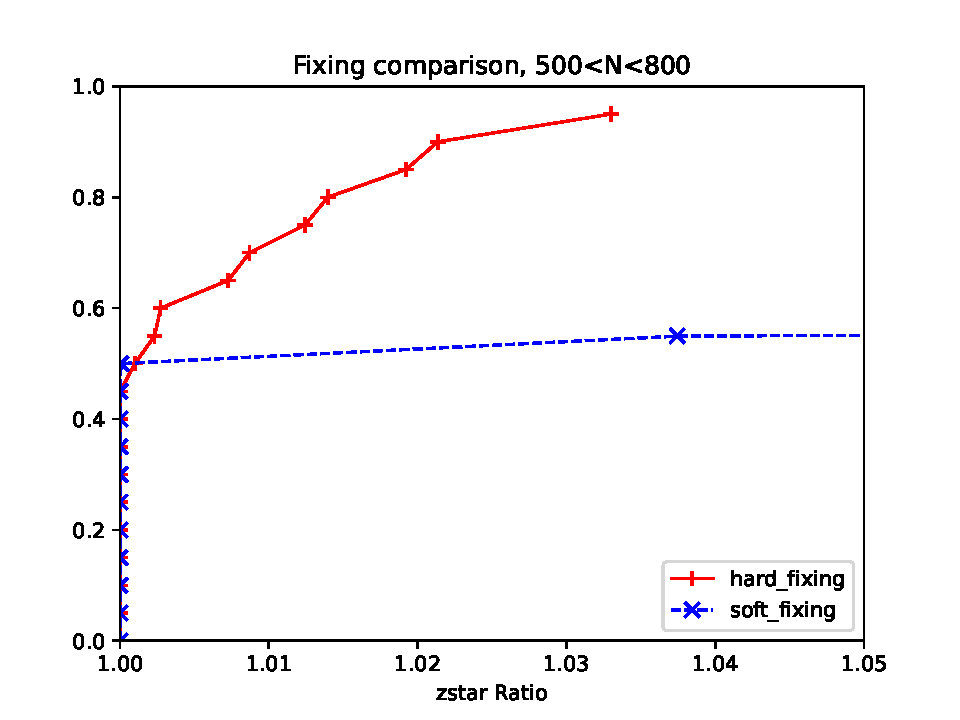
\includegraphics[width=0.8\linewidth]{figures/math}
        \caption{Matheuristics comparison}
\end{figure}

The comparison is done using random generated instances with a number of nodes
between 500 and 800 running for around 12 minutes each. The results showed that
hard fixing is quite consistent in returning a good solution even if it starts
with a bad one. In most of the cases it returns a solution within 2-3\% of the
optimum. Soft fixing, instead, strongly depends on the starting solution as we
expected. In fact, as stated before, in the hyperparameters tuning phase it
turned out that it was better to leave more time for the first iteration. It is
very clear observing the differences on how instances are solved. Almost every
time soft fixing find a good solution at the beginning it is better than hard
fixing and it comes very close to the optimal solution. As you can see they
split almost equally the victories but only once the loser solution of soft
fixing is close. Instead, all the times hard fixing is competitive. In fact,
when both start with a bad solution hard fixing manage to reach a good
approximation within the given timelimit, while for soft fixing is not the
case. When timelimit is too small it is a valid option starting with a k higher
than 3 because otherwise most of the iteration will lead to a very small change
consuming a significant part of the time.     
